\documentclass[../main.text]{subfiles}

In this section I develop a simple differences-in-differences estimate of the effect of the City Council's revision of the camping ban on crime. I aggregate both crime data and citation data at the census tract level on a monthly basis to create a balanced panel of \(T = 60\) months and \(N=113\) census tracts. I define a treatment cutoff \(q_{D}\) as the 90th percentile of the citations pre-treatment:
\begin{equation*}
    q_{D} = G_{(.9)};\; G = \left\{ \frac{1}{t^*}\sum_{t = 1}^{t^*} x_{it} \;\big|\; i = 1,\dots,N \right\}
\end{equation*}
Here, \(x_{it}\) is the number of camping ordinance citations in census tract \(i\) in month \(t\). I let \(t^*\) represent the treatment date—I will present results using both June 28, 2018 and June 20, 2019 as treatment dates.

Next, I assign a treatment to each census tract \(i\), \(D_i\), based on the treatment cutoff \(q_{D}\):
\begin{equation*}
    D_i = 1\left( \frac{1}{t^*}\sum_{t = 1}^{t^*} x_{it} > q_{D} \right)
\end{equation*}
Given my assumed correspondence between the number of citations given, the number of unsheltered people, and the transience of the deterrent effect, treated census tracts represent the areas of the city with the largest homeless populations. A map of Austin with treated areas shaded is in Figure~\ref{fig:treatment_by_tract}.

Letting \(S_t = 1(t > t^*)\), I construct the model
\begin{equation*}
    y_{it} = \theta_0 + \theta_1 S_t + \theta_2 D_i + \delta (D\times S)_{it} + \alpha_i + \varepsilon_{it}
\end{equation*}
The outcome \(y_{it}\) is the number of crime reports in census tract \(i\) in month \(t\). I let \(\alpha_i\) control for unobserved time-invariant heterogeneity in tract \(i\), with \(\varepsilon_{it}\) mean-independent error. The coefficient of interest is \(\delta\), which measures the mean change in monthly crime reports in affected areas of the city post ordinance reform.

\begin{figure}
    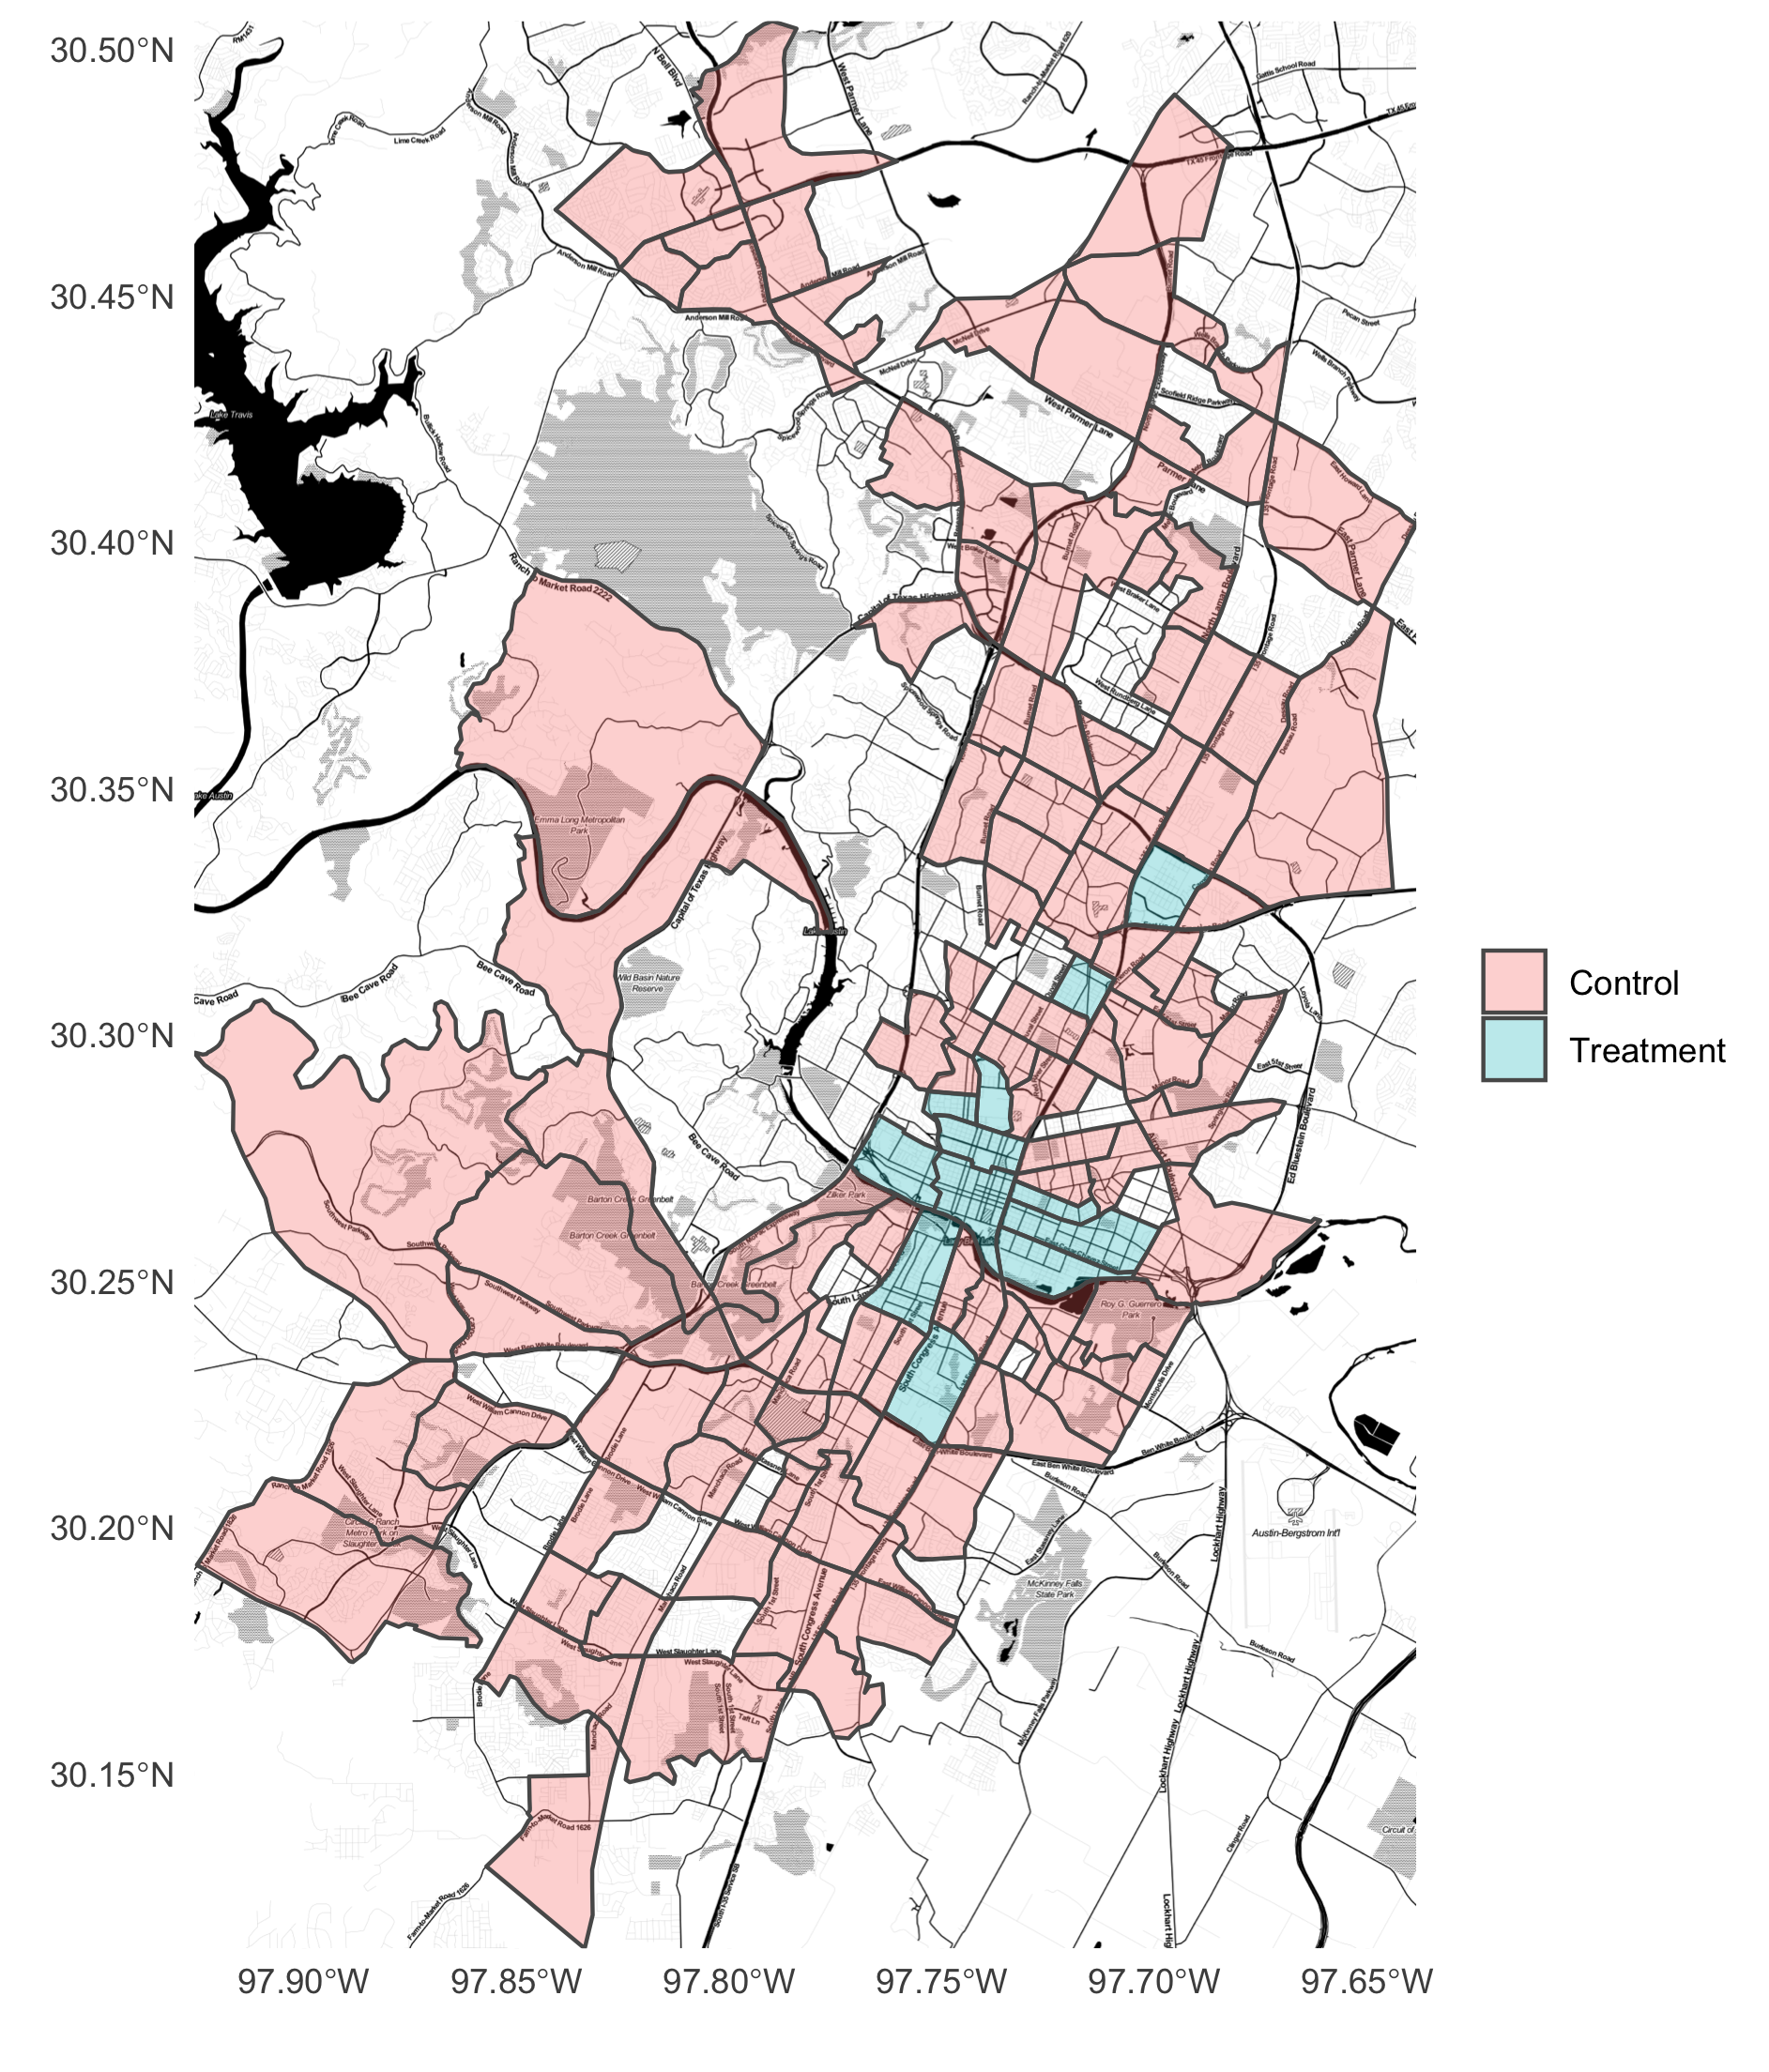
\includegraphics[width=\textwidth]{../../figures/treatment_by_tract.png}
    \caption{Map of treated and control areas of Austin according to pre-treatment citation levels. Note the main treated areas are near Downtown Austin and the University of Texas.}
    \label{fig:treatment_by_tract}
\end{figure}


\begin{table}
    \begin{center}
        
\begin{tabular}{ccc}
    Cutoff Date     &   Estimate   &   Std Error \\ \toprule
    June 28, 2018   &   3.1285164        &   2.584715 \\
    June 20, 2019   &   3.5410402        &   2.8821456 \\ \bottomrule
\end{tabular}

    \end{center}
    \caption{Point estimates and bootstrap standard errors of OLS DID estimate}
    \label{tab:did_1}
\end{table}

\subsection{Identifying Assumptions}

In order to identify our model we must make both the typical strict exogeneity assumption of a fixed-effect model and the parallel trends assumption of a difference-in-difference model. Conditional on the tract-level fixed effect, we are assuming that 